\documentclass[12pt, letterpaper, oneside]{book}

%\usepackage{fullpage}
%\usepackage{anysize}
%\marginsize{3.6cm}{2.54cm}{2.54cm}{2.54cm} %iz, der, arriba, abajo
\usepackage[top=2.54cm, bottom=2.54cm, left=3.6cm, right=2.54cm,headsep=10pt]{geometry}

\usepackage[utf8]{inputenc}
\parindent0cm %nuevo

%\usepackage{multicol} % This is so we can have multiple columns of text side-by-side
%\columnsep=20pt % This is the amount of white space between the columns in the poster
%\columnseprule=0pt % This is the thickness of the black line between the columns in the poster

\usepackage[svgnames]{xcolor} % Specify colors by their 'svgnames', for a full list of all colors available see here: http://www.latextemplates.com/svgnames-colors

\usepackage{times} % Use the times font
%\usepackage{palatino} % Uncomment to use the Palatino font

\usepackage{graphicx} % Required for including images
%\usepackage{background}
\usepackage{transparent}

\graphicspath{{figures/}} % Location of the graphics files
\graphicspath{ {images/} }
\usepackage{float}
\usepackage{mathdots} % para el comando \iddots
\usepackage{mathrsfs} % para formato de letra
\usepackage{amssymb, amsmath, amsbsy} % simbolitos
\usepackage{booktabs} % Top and bottom rules for table
\usepackage[font=small,labelfont=bf]{caption} % Required for specifying captions to tables and figures
\usepackage{amsfonts, amsmath, amsthm, amssymb} % For math fonts, symbols and environments
\usepackage{wrapfig} % Allows wrapping text around tables and figures
\usepackage{listings}
\usepackage{matlab-prettifier}%PARA INSERTAR CODIGOS DE MATLAB
%\usepackage[latin1]{inputenc}
\usepackage[spanish]{babel}
\usepackage{setspace}
\usepackage{amsmath}
\usepackage{amsthm}
\usepackage{amssymb}

\usepackage{titletoc} %nuevo
\usepackage{afterpage} %nuevo
%\usepackage[breaklinks=true]{hyperref} %nuevo
\usepackage[hidelinks]{hyperref} %nuevo
\usepackage{multirow, array}
%\usepackage[nottoc]{tocbibind}
%\usepackage[nottoc,numbib]{tocbibind}

%%%%%%%%%%%%%%%%%%%%%%%%%%%%%%%%%%%%%%%%%%%%% Pie de pagina
\usepackage{fancyhdr} % Cabeceras/Pies
\pagestyle{fancy} % Cabeceras/Pies
\usepackage{lastpage}



%\providecommand\phantomsection{}

\begin{document}
\pagenumbering{roman}

\begin{titlepage}
	\centering
	
\includegraphics[width=6cm]{figures/logo_universidad.png}\par \vspace{2cm}
	{\textbf{\LARGE Titulo del trabajo de grado o asistencia de investigacion} \par}
	\vspace{7cm}
	{\Large \textbf{Nombre del autor} \par}
	\vfill %\vspace{7cm}
	{\normalsize \textbf{Facultad del programa} \par}
	{\normalsize \textbf{Programa } \par}
	{\normalsize ciudad, año \par}
\end{titlepage}
\afterpage{\null\newpage}
\newpage
\thispagestyle{empty}

\begin{center}
%\newpage{\pagestyle{empty}\cleardoublepage}
%\newpage
\thispagestyle{empty} \vspace*{1cm}
\textbf{\LARGE
Titulo del trabajo de grado o asistencia de investigación}\\[3.0cm]
\Large\textbf{Nombre del autor}\\[3.0cm]
\small Trabajo de grado presentado como requisito parcial para optar al
t\'{\i}tulo de:\\
\textbf{programa o titulo}\\[2.5cm]
Director(a):\\
Ph.D, Msc o titulo, nombre del director\\
Profesor de:\\\vfill
Facultad del programa\\
Programa \\
ciudad, año\\
\end{center}
\afterpage{\null\newpage}
\newpage
\thispagestyle{empty}


\chapter*{Dedicatoria}

Su uso es opcional y cada autor podrá determinar la distribución del texto en la página, se sugiere esta presentación. En ella el autor del trabajo dedica su trabajo en forma especial a personas y/o entidades
\afterpage{\null\newpage}
\newpage
\thispagestyle{empty}

\chapter*{Agradecimientos}

Esta sección es opcional, en ella el autor agradece a las personas o instituciones que colaboraron en la realización del trabajo. Si se incluye esta sección, deben aparecer los nombres completos, los cargos y su aporte al trabajo.
  

\chapter*{Resumen}
\addcontentsline{toc}{chapter}{Resumen\dotfill}

El resumen es una presentación abreviada y precisa. Se recomienda que este resumen sea analítico, es decir, que sea completo, con información cuantitativa y cualitativa, generalmente incluyendo los siguientes aspectos: objetivos, diseño, lugar y circunstancias, objetivo del estudio, intervención, mediciones y principales resultados, y conclusiones. Extensión máxima sugerida: 12 renglones\\

\textbf{Palabras clave:} (máximo 7 palabras, preferiblemente seleccionadas de las listas internacionales que permitan el indizado cruzado). 

\section*{Abstract}

Es el mismo resumen pero traducido al inglés.\\

\textbf{Keywords} (palabras clave en ingles). 


 

\thispagestyle{empty}
\renewcommand{\tablename}{\textbf{Tabla}}
\renewcommand{\figurename}{\textbf{Figura}}
\renewcommand{\listtablename}{Lista de Tablas}
\renewcommand{\listfigurename}{Lista de Figuras}

%\cleardoublepage
%\phantomsection
%\addcontentsline{toc}{chapter}{Resumen\dotfill}

{\renewcommand{\contentsname}{Contenido}\tableofcontents}


\cleardoublepage
\phantomsection
\addcontentsline{toc}{chapter}{Lista de figuras\dotfill} % para que aparezca en el indice de contenidos
\listoffigures % indice de figuras

\cleardoublepage
\phantomsection
\addcontentsline{toc}{chapter}{Lista de tablas\dotfill} % para que aparezca en el indice de contenidos
\listoftables % indice de tablas

\cleardoublepage
\phantomsection
\addcontentsline{toc}{chapter}{Introduccion\dotfill}


\pagestyle{fancyplain}
\renewcommand{\headrulewidth}{0.4pt}
%\lhead{\transparent{0.2}\includegraphics[scale=0.1]{figures/Unibague_ESCUDO.jpg}} 
\lfoot{Proyecto de grado, año}
\cfoot{} 
\rfoot{\thepage/\pageref{LastPage}} 
\renewcommand{\footrulewidth}{0.4pt}

\pagenumbering{arabic}
\markboth{INTRODUCCIÓN}{}
\thispagestyle{fancyplain}
\chapter*{Introducción}


En la introducción, el autor presenta y señala la importancia, el origen (los antecedentes teóricos y prácticos), los objetivos, los alcances, las limitaciones, la metodología empleada, el significado que el estudio tiene en el avance del campo respectivo y su aplicación en el área investigada. No debe confundirse con el resumen y se recomienda que la introducción tenga una extensión de mínimo 2 páginas y máximo de 4 páginas.\\

La presente plantilla maneja la fuente Arial para el texto de los párrafos y para los títulos y subtítulos. Sin embargo, es posible sugerir otras fuentes tales como Garomond, Calibri, Cambria o Times New Roman, que por claridad y forma, son adecuadas para la edición de textos académicos.\\ 

Esta sección se encabeza con la palabra introducción, escrita con minúscula (en la primera línea), con un espaciado anterior de 30 puntos y posterior de 10 puntos, interlineado sencillo y en letra negrilla de 20 puntos (en este caso se usa Arial).\\

La presente plantilla tiene en cuenta los aspectos generales recomendados por la Norma Técnica Colombiana - NTC 1486, con el fin que sea usada para la presentación final de los trabajos finales de grado de los programas académicos (en cualquiera de sus modalidades o sus niveles de formación) de la Facultad de Ingeniería, desarrollados en la Universidad de Ibagué en Colombia.\\

Las márgenes deben ser de 2,54 centímetros (1 pulgada) en la parte superior, inferior y exterior y de 3,6 centímetros en la margen interna (a partir de márgenes simétricos). La plantilla está diseñada para imprimir por lado y lado en hojas tamaño carta, y está construida por secciones (Capítulo 1, Capítulo 2, Capitulo 3, Capítulo 4, Capitulo 5,). El encabezado de las páginas impares contendrá el título del trabajo en letra Arial 8 puntos, el encabezado en las páginas pares contendrá la sección que se desarrolla. En el pie de página se ubica además del número de página, el nombre de los autores en páginas impares y el nombre del programa -tipo de trabajo- año de presentación, en las páginas pares (en letra Arial de 8 puntos, de acuerdo al formato presentado en esta plantilla). \\

El título de cada capítulo debe estar numerado y comenzar en una hoja independiente (página impar) y con el mismo formato del título Introducción (escrita con minúscula, en la primera línea, con un espaciado anterior de 30 puntos y posterior de 10 puntos e interlineado 1.15 y en letra de 16 puntos y negrilla. El texto debe llegar hasta la margen inferior establecida. Se debe evitar títulos o subtítulos solos al final de la página o renglones sueltos. \\

Si se requiere ampliar la información sobre normas adicionales para la escritura se puede consultar la norma NTC 1486 en la Base de datos del ICONTEC (Normas Técnicas Colombianas) disponible en el portal del SINAB de la Universidad Nacional de Colombia www.sinab.unal.edu.co, en la sección “Recursos bibliográficos” opción “Bases de datos”.  Este portal también brinda la posibilidad de acceder a un instructivo para la utilización de Microsoft Word y Acrobat Professional.\\

La tesis o trabajo de investigación se debe escribir con interlineado 1.15 y después de punto aparte a una interlínea (una veces la tecla Enter). La redacción debe ser impersonal y genérica. La numeración de las hojas sugiere que las páginas preliminares se realicen en números romanos en mayúscula y las demás en números arábigos, en forma consecutiva a partir de la introducción que comenzará con el número 1. La cubierta y la portada no se numeran pero si se cuentan como páginas.\\

El tamaño de letra sugerido y teniendo en cuenta la familia fuente Arial de 11 puntos para el texto de estilo “Párrafo”, Arial para los títulos, de 16 puntos (estilo “Título Primer nivel”) y de 14 y 12 para los subtítulos (estilos “Título segundo nivel” y “Título tercer nivel”, respectivamente). \\

La extensión máxima de un documento de trabajo de grado, se sugiere en no más de 50 páginas en programas de pregrado y en no más de 60 páginas en programas de posgrado, sin considerar páginas de anexos ni preliminares.\\

No se debe utilizar una numeración adicional a la que es propia de la tabla de contenido. Tampoco utilice numeración compuesta como 13A, 14B ó 17 bis.  Si requiere hacer enumeración dentro de apartados, utilice viñetas ( $\blacksquare$ ) o números romanos en minúscula (i, ii, etc). Los Anexos se indican con letras alfabéticas en mayúscula, según su orden de llamado en el texto (Anexo A, etc.). \\

Para resaltar, puede usarse letra cursiva o negrilla. Los términos de otras lenguas que aparezcan dentro del texto se deben escribir en cursiva.\\
 

\thispagestyle{empty}
\afterpage{\null\newpage}
\newpage

%\mainmatter

\chapter{Nombre del capitulo}

Los capítulos son las principales divisiones del documento. En estos se desarrolla el tema del documento. Cada capítulo debe corresponder a uno de los temas o aspectos considerados dentro del proyecto que dio lugar al trabajo de grado.  El interlineado de texto en capítulos es de 1.15.

\section{Subtítulos nivel 2}
Toda división o capítulo, a su vez, puede subdividirse en otros niveles y sólo se enumera hasta el tercer nivel. Los títulos de segundo nivel se escriben con minúscula al margen izquierdo y sin punto final, están separados del texto o contenido por un interlineado posterior de 10 puntos y anterior de 20 puntos (tal y como se presenta en la plantilla).

\subsection{Subtítulos nivel 3}

De la cuarta subdivisión en adelante, cada nueva división o ítem puede ser señalada con viñetas, conservando el mismo estilo de ésta, a lo largo de todo el documento.\\

\begin{itemize}
\item En caso que sea necesario utilizar viñetas, use este formato (viñetas cuadradas).
\end{itemize}

Las subdivisiones, las viñetas y sus textos acompañantes deben presentarse sin sangría y justificados. 

\begin{figure}[h]
\centering

\includegraphics[scale=0.5]{../figures/logo_universidad.png}
\caption{ejemplo imagen}
\end{figure}


 


\chapter{}

Existen varias normas para la citación bibliográfica. Algunas áreas del conocimiento prefieren normas específicas para citar las referencias bibliográficas en el texto y escribir la lista de bibliografía al final de los documentos. Esta plantilla brinda la libertad para que el autor de la tesis utilice la norma bibliográfica común para su disciplina. Sin embargo, se solicita que la norma seleccionada se utilice con rigurosidad, sin olvidar referenciar “todos” los elementos tomados de otras fuentes (referencias bibliográficas, patentes consultadas, software empleado en el manuscrito, en el tratamiento a los datos y resultados del trabajo, consultas a personas (expertos o público general), entre otros).

\section{Ejemplos de citaciones bibliográficas}

Existen algunos ejemplos para la citación bibliográfica, por ejemplo, Microsoft Word (versiones posteriores al 2006), en el  menú de referencias, se cuenta con la opción de insertar citas bibliográficas utilizando la norma IEEE (Institute of Electrical \& Electronic Engineers) APA (American Psychological Association) u otras normas construir automáticamente la lista al final del documento. De la misma manera, existen administradores bibliográficos compatibles con Microsoft Word como Zotero, Mendelley, End Note y el Reference Manager. \\

Por lo general, las referencias bibliográficas se listan al final del documento en orden de aparición (caso de IEEE) o en orden alfabético (caso de APA e ICONTEC). 
A continuación se muestra un ejemplo de la citación en texto de las formas más usadas para las citaciones bibliográficas en ciencias de la Ingeniería: \\

Citación individual: [3].
Citación simultánea de varios autores: [1, 12, 9, 14, 6, 11, 5, 8, 2, 13, 4]\\

Bajo la norma IEEE solo se refiere el número  encerrado en corchetes  [  ], por ejemplo 1) “…énfasis en elementos ligados al ámbito ingenieril que se enfocan en el manejo de datos e información estructurada y que según Kostoff [3] ha atraído la atención de investigadores dado el advenimiento de TIC..”, 2) “…Dicha afirmación coincide con los planteamientos de Snarch, citado por Castellanos [4], quien comenta que el manejo…” y 3)  “…el futuro del sistema para argumentar los procesos de toma de decisiones y el desarrollo de ideas innovadoras…”.[5].

Las normas de citación en texto de APA incluyen el apellido del autor y el año de la referencia, por ejemplo estas son las opciones 1) “…énfasis en elementos ligados al ámbito ingenieril que se enfocan en el manejo de datos e información estructurada y que según Kostoff (1997) ha atraído la atención de investigadores dado el advenimiento de TIC..”, 2) “…Dicha afirmación coincide con los planteamientos de Snarch (1998), citado por Castellanos (2007), quien comenta que el manejo…” y 3)  “…el futuro del sistema para argumentar los procesos de toma de decisiones y el desarrollo de ideas innovadoras (Nosella et al., 2008)…”.\\


\section{Ejemplos de presentación y citación de figuras}

Las ilustraciones forman parte del contenido de los capítulos. Se deben colocar en la misma página en que se mencionan o en la siguiente (deben siempre mencionarse en el texto). No se debe emplear la abreviatura "No." ni el signo "\#" para su numeración. \\

Las llamadas para explicar algún aspecto de la información deben hacerse con nota al pie y su nota correspondiente \footnote{Las notas van como “notas al pie”, con interlineado sencillo, el texto justificado y usando la letra del texto en 10 puntos. Se utilizan para explicar, comentar o hacer referencia al texto de un documento, así como para introducir comentarios detallados y en ocasiones para citar fuentes de información (aunque para esta opción es mejor seguir en detalle las normas de citación bibliográfica seleccionadas).} . La fuente documental se debe escribir al final de la ilustración o figura con los elementos de la referencia (de acuerdo con las normas seleccionadas) y no como pie de página. Un ejemplo para la presentación y citación de figuras, se presenta a continuación (citación directa):\\

Por medio de las propiedades del fruto, según el espesor del endocarpio, se hace una clasificación de la palma de aceite en tres tipos: Dura, Ternera y Pisifera, que se ilustran en la Figura 2 1. \\


\begin{figure}[hbtp]
\centering
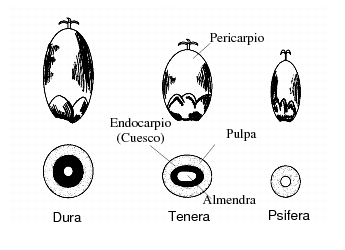
\includegraphics[scale=1]{../figures/figura.png}
\caption{Tipos y partes de la semilla de  palma de aceite, fuente}
\cite{AG03p,AG04p}
\end{figure}





\section{Citación de tablas y cuadros}
%\markboth{}{}

Para la edición de tablas, cada columna debe llevar su título; la primera palabra se debe escribir con mayúscula inicial y preferiblemente sin abreviaturas. En las tablas y cuadros, los títulos y datos se deben ubicar entre líneas horizontales y verticales cerradas.\\

La numeración de las tablas se realiza de la misma manera que las figuras o ilustraciones, a lo largo de todo el texto. Deben llevar un título breve, que concreta el contenido de la tabla; éste se debe escribir en la parte superior de la misma. Para la presentación de cuadros, se deben seguir las indicaciones dadas para las tablas.\\

Un ejemplo para la presentación y citación de tablas (citación indirecta), se presenta a continuación:

De esta participación aproximadamente el 60 \% proviene de biomasa (ver Tabla 2 1).\\

\begin{table}[h]
\centering
\begin{tabular}{|l|c|c|} 
\hline
\multirow{2}{*}{Región} & \multicolumn{2}{l|}{Participación de suministros de energía primaria}                                                                 \\ 
\cline{2-3}
                        & \begin{tabular}[c]{@{}c@{}}Energías \\Renovables\end{tabular} & \begin{tabular}[c]{@{}c@{}}Participación\\de la biomasa\end{tabular}  \\ 
\hline
Latinoamerica           & 28,9                                                          & 62,4                                                                  \\ 
\hline
Colombia                & 27,7                                                          & 54,4                                                                  \\ 
\hline
Alemania                & 3,8                                                           & 65,8                                                                  \\ 
\hline
Mundial                 & 13,1                                                          & 79,4                                                                  \\
\hline
\end{tabular}
\caption{Participación de las energías renovables primarias, fuente.}
\end{table}

\subsection{Consideraciones adicionales para el manejo de figuras y tablas}

Cuando una tabla o cuadro ocupa más de una página, se debe repetir su identificación numérica, seguida por la palabra continuación, con mayúscula inicial, entre paréntesis, como el siguiente ejemplo.\\

\textbf{Tabla 1-1:} 	(Continuación)

Adicional mente los encabezados de las columnas se deben repetir en todas las páginas después de la primera. 

\begin{itemize}
\item Ejemplo de presentación y citación de ecuaciones
\end{itemize}  

Un ejemplo para la presentación y citación de ecuaciones, se presenta a continuación: … de esta forma, el punto de partida es una ecuación de velocidad, independiente de los cambios a nivel interno del carbonizado que afectan la reacción, constituida por dos términos dependientes de la temperatura de gasificación y del medio gasificante, respectivamente, y a su vez independientes entre sí (ver Ecuación (2.1)).

\begin{equation}
-r=-\frac{dW_C/dt}{W_C}=f\left(T_G\right).f(C_{H_2O})
\end{equation}

Para el manejo de cifras y siglas, oriéntese por el Sistema Internacional de Medidas (mayor información en http://www.sc.ehu.es)\\ 

Sólo refiera las fuentes de tablas y figuras, si estás corresponden a un origen diferente al trabajo de los autores del estudio que se reporta, o si han sido adaptadas de una fuente externa. \\

Puede utilizar colores a la escala de grises, sólo en los casos que las figuras así lo demanden para comprensión de contenido. También puede utilizar un sombreado suave en los encabezados de tablas, para distinguirlos de su contenido. En todo caso, el estilo que utilice en las tablas, debe ser el mismo en todos los capítulos.\\ 

En el caso de figuras resultantes de análisis estadísticos o similares, deben quedan debidamente identificados: significado de ejes, unidades de medida, nombre de series, horizonte de tiempo (si aplica).\\


\chapter{capitulo 3}

Se deben incluir tantos capítulos como se requieran; sin embargo, se recomienda que la tesis o trabajo de investigación tenga un mínimo 3 capítulos y máximo de 6 capítulos (incluyendo las conclusiones).
\chapter{Capitulo 4}

Se deben incluir tantos capítulos como se requieran; sin embargo, se recomienda que la tesis o trabajo de investigación tenga un mínimo 3 capítulos y máximo de 6 capítulos (incluyendo las conclusiones).
\chapter{Conclusiones y Recomendaciones}
\section{Conclusiones}

Las conclusiones constituyen un capítulo independiente y presentan, en forma lógica, los resultados del trabajo. Las conclusiones deben ser la respuesta a los objetivos o propósitos planteados. Se deben titular con la palabra conclusiones en el mismo formato de los títulos de los capítulos anteriores (Títulos primer nivel), precedida por el numeral correspondiente (según la presente plantilla). \\

Las conclusiones deben contemplar las perspectivas de la investigación, las cuales son sugerencias, proyecciones o alternativas que se presentan para modificar, cambiar o incidir sobre una situación específica o una problemática encontrada. Pueden presentarse como un texto con características argumentativas, resultado de una reflexión acerca del trabajo de investigación. 


\section{Recomendaciones}

Se presentan como una serie de aspectos que se podrían realizar en un futuro para emprender investigaciones similares o fortalecer la investigación realizada.

\section{bibliografia}
%\markboth{}{}

Existen algunos ejemplos para la citaci\'{o}n bibliogr\'{a}fica, por ejemplo, Microsoft Word (versiones posteriores al 2006), en el  men\'{u} de referencias, se cuenta con la opci\'{o}n de insertar citas bibliogr\'{a}ficas utilizando la norma APA (American Psychological Association) u otras normas y con la ayuda para construir autom\'{a}ticamente la lista al final del documento. De la misma manera, existen administradores bibliogr\'{a}ficos compatibles con Microsoft Word como Zotero, End Note y el Reference Manager,  disponibles a trav\'{e}s del Sistema Nacional de Bibliotecas (SINAB) de la Universidad Nacional de Colombia secci\'{o}n "Recursos bibliogr\'{a}ficos" opci\'{o}n "Herramientas Bibliogr\'{a}ficas. A continuaci\'{o}n se muestra un ejemplo de una de las formas m\'{a}s usadas para las citaciones bibliogr\'{a}ficas.\\

Citaci\'{o}n individual:\cite{AG01}.\\
Citaci\'{o}n simult\'{a}nea de varios autores:
\cite{AG12,AG52,AG70,AG08a,AG09a,AG36a,AG01i}.\\

Por lo general, las referencias bibliogr\'{a}ficas correspondientes a los anteriores n\'{u}meros, se listan al final del documento en orden de aparici\'{o}n o en orden alfab\'{e}tico. Otras normas de citaci\'{o}n incluyen el apellido del autor y el a\~{n}o de la referencia, por ejemplo: 1) "...\'{e}nfasis en elementos ligados al \'{a}mbito ingenieril que se enfocan en el manejo de datos e informaci\'{o}n estructurada y que seg\'{u}n Kostoff (1997) ha atra\'{\i}do la atenci\'{o}n de investigadores dado el advenimiento de TIC...", 2) "...Dicha afirmaci\'{o}n coincide con los planteamientos de Snarch (1998), citado por Castellanos (2007), quien comenta que el manejo..." y 3) "...el futuro del sistema para argumentar los procesos de toma de decisiones y el desarrollo de ideas innovadoras (Nosella \textsl{et al}., 2008)...".\\


En esta sección de relacionan las fuentes documentales consultadas por el estudiante o investigador para sustenta su trabajo. Su inclusión es obligatoria. Cada referencia bibliográfica se inicia contra el margen izquierdo, y puede presentarse con interlineado sencillo. \\

La Universidad acepta las siguientes tres normas para manejo de referencias: 

\begin{center}
\begin{table}[H]
\centering
\begin{tabular}{|p{2cm}|p{3cm}|p{6cm}|}
\hline
Institución	&	Disciplina de aplicación	& Vínculos y ejemplos \\ 
\hline
NTC 5613	&	varias	&	ICONTEC	\\ 
\hline
American Psychological Association (APA)                   & Común en ciencias de la salud, sociales, humanidades y administración. & APAStyle.org.
\hspace{0.1cm}
Biblioteca.udg.es/Info\ \_General/Guies/Cites/Citar\ 
\_Llibres.asp (reglamento). 
Liunet.edu/Cwis/Cwp/
Library/Workshop/Citapa.htm (ejemplos).  \\ 
\hline
Institute of Electrical and Electronic Engineers (IEEE) & Ciencias
básicas y técnicas (Ingenierías)	& IEEE	\\
\hline
\end{tabular}
\end{table}
\end{center}

Para incluir las referencias dentro del texto y realizar lista de la bibliografía en esta sección, puede utilizar las herramientas de Microsoft Word para Citas y bibliografía en la pestaña de Referencias, utilizar administradores bibliográficos o, revisar el instructivo desarrollado por el Sistema de Bibliotecas de la Universidad Nacional de Colombia www.sinab.unal.edu.co, disponible en la sección “Servicios”, opción “Trámites” y enlace “Entrega de tesis”.

Por ultimo se tomo como documento de apoyo la plantilla brindada por la Universidad Nacional en su portal "sinab" \cite{sinab}, mediante el cual se logro desarrollar esta plantilla personalizada.


{\bibliographystyle{ieeetr}\bibliography{Componentes/Bibliografia}}
\addcontentsline{toc}{chapter}{Bibliografia\dotfill}

\begin{appendix}
\chapter{Anexo: Nombrar el anexo A de acuerdo con su contenido}\label{AnexoA}
Los Anexos son documentos o elementos que complementan el cuerpo de la tesis o trabajo de investigaci\'{o}n y que se relacionan, directa o indirectamente, con la investigaci\'{o}n, tales como acetatos, cd, normas, etc.\\

\chapter{Anexo: Nombrar el anexo B de acuerdo con su contenido}
A final del documento es opcional incluir \'{\i}ndices o glosarios. \'{E}stos son listas detalladas y especializadas de los t\'{e}rminos, nombres, autores, temas, etc., que aparecen en el mismo. Sirven para facilitar su localizaci\'{o}n en el texto. Los \'{\i}ndices pueden ser alfab\'{e}ticos, cronol\'{o}gicos, num\'{e}ricos, anal\'{\i}ticos, entre otros. Luego de cada palabra, t\'{e}rmino, etc., se pone coma y el n\'{u}mero de la p\'{a}gina donde aparece esta informaci\'{o}n.\\

\chapter{Anexo: Nombrar el anexo C de acuerdo con su contenido}
MANEJO DE LA BIBLIOGRAF\'{I}A: la bibliograf\'{\i}a es la relaci\'{o}n de las fuentes documentales consultadas por el investigador para sustentar sus trabajos. Su inclusi\'{o}n es obligatoria en todo trabajo de investigaci\'{o}n. Cada referencia bibliogr\'{a}fica se inicia contra el margen izquierdo.\\


\end{appendix}


%\renewcommand{\refname}{}	

\end{document}




